\section{Experiments}
\subsection{Experimental Setup}
\label{sec:baseline_rag_systems}
\paragraph{Baseline RAG Systems}
We apply \benchname\space to 8 customized RAG systems to demonstrate how these metrics reflect the properties and differences among them, and how they guide the refinement of these systems. The 8 RAG systems are combinations with 2 retrievers and 4 generators. For retrievers, we choose BM25~\cite{robertson2009probabilistic}, a representative classic sparse retrieval framework, and E5-Mistral~\cite{wang2023improving}, the SOTA open-source dense retriever. Our four generators are GPT-4~\cite{openai2023gpt4}, Mixtral-8x7B~\cite{jiang2024mixtral}, Llama3-8B, and Llama3-70B~\cite{llama3modelcard}, covering open-source and proprietary LLMs in various sizes. Further details are deferred to Appendix~\ref{appendix:experiment_setup_detail}. 
We employ Llama3-70B as both the claim extractor and checker models implemented by an open-sourced framework RefChecker\footnote{\url{https://github.com/amazon-science/RefChecker}}~\cite{hu2024refchecker}. As a validation of its performance on the RefChecker's hallucination detection benchmark, this setup outperforms the best purely open-sourced combinations reported in RefChecker's paper (see Appendix~\ref{appendix:refchecker_validation}).

\paragraph{Benchmark Datasets}

For comprehensive evaluations, we curate a benchmark containing 4,162 queries across 10 domains. This benchmark is repurposed from public datasets of open domain question answering, spanning domains of Wikipedia, AI science, novel, biomedical, finance, lifestyle, recreation, science, technology and writing. We convert the short answers to long-form answers in the datasets to align with the current LLM-based RAG systems. Please refer to Appendix~\ref{appendix:benchmark} for the details of the benchmark curation process. The statistics of the benchmark are shown in Tab.~\ref{tab:benchmark_stat}.


\begin{table}[]
    \centering
    \renewcommand{\arraystretch}{1.5}
    \caption{Statistics of the RAG benchmark. This benchmark is repurposed from  public datasets across 10 domains, containing 4,162 questions. For the domains of Finance, Lifestyle, Recreation, Technology, Science and Novel, the short answers are extended to long-form answers with GPT-4.}
    \label{tab:benchmark_stat}
    \scalebox{0.85}{
    \begin{tabular}{>{\arraybackslash}m{1.8cm}
    >{\centering\arraybackslash}m{1.5cm}
    >{\centering\arraybackslash}m{1.2cm}
    >{\centering\arraybackslash}m{1.5cm}
    >{\centering\arraybackslash}m{1.5cm}
    >{\centering\arraybackslash}m{6cm}}
\toprule
\textbf{Dataset} & \textbf{Domain} & \textbf{\# Query} & \textbf{\# Doc.} & \textbf{Source} & \textbf{Example Query} \\
\hline
ClapNQ & Wikipedia & 300 & 4,293 & ClapNQ & Difference between russian blue and british blue cat \\\hline
NovelQA & Novel & 280 & 19 & NovelQA & When do the Ewell kids go to school? \\\hline
RobustQA Writing & Writing & 500 & 199,994 & LoTTE, RobustQA & What is the difference between online and internet? \\\hline
RobustQA BioASQ & Biomedical & 511 & 197,816 & BioASQ & What hand deformities do patients with Apert syndrome present with? \\\hline
RobustQA Finance & Finance & 500 & 57,638 & FiQA, RobustQA & Is it safer to send credit card number via unsecured website form or by e-mail? What safer options are there? \\\hline
RobustQA Lifestyle & Lifestyle & 500 & 119,461 & LoTTE, RobustQA & Can i eat a day old peanut butter sandwich? \\\hline
RobustQA Recreation & Recreation & 500 & 166,975 & LoTTE, RobustQA & Why are so many american (spy) movies set in europe? \\\hline
RobustQA Science & Science & 500 & 125,368 & LoTTE, RobustQA & Where is the flaw in this proof that 1=2? (derivative of repeated addition) \\\hline
RobustQA Technology & Technology & 500 & 638,509 & LoTTE, RobustQA & Why not use larger cipher keys? \\\hline
KIWI & AI Science & 71 & 429 & KIWI & What are the prior approaches proposed to improve faithfulness of the reasoning steps generated by LLMs and what tasks are they applied on? \\
\bottomrule
    \end{tabular}
    }
% \label{tab:datasets}
\end{table}

% \textbf{Retrievers}
% BM25 ranks documents based on term frequency, inverse document frequency, and document length statistics. As a classic matching algorithm derived from the probabilistic retrieval framework~\cite{robertson2009probabilistic}, it is widely adopted for its simplicity, robustness across various domains, and high efficiency with inverted index. E5-Mistral \cite{wang2023improving} is a text embedding model, fine-tuned from the decoder-only language model (Mistral-7B-Instruct) using labeled retrieval data and synthetic data generated by proprietary LLMs. It ranks documents based on cosine similarities between document embeddings and query embeddings, representing the SOTA in open-source dense retrieval.

% \textbf{Generators}
% The four generators include GPT-4 \cite{xx}, representing advanced proprietary LLMs; Llama3 \cite{llama3}, as strong open-source models for comparison; and Mixtral-8x7B \cite{jiang2024mixtral}, as a typical mixture-of-experts model. For Llama3, we use both the 8B and 70B versions to study the impact of model size within the same family.

% \textbf{RAG Systems}
% We adopt OpenSearch \cite{xx} as the tool to implement the inverted index for BM25 and approximate KNN search for dense retrieval. We split documents in the corpus to chunks of 300 tokens with an overlap ratio of 0.2 by default. We use the tokenizer of E5-Mistral for both retrievers to control the chunking. For each query, top-20 chunks ranked by retrievers are used as context for LLM generation. The default generation prompt is shwon in Appendix~\ref{xx}.
% \begin{tcolorbox}[colback=OliveGreen!5!white,colframe=teal!75!black]
% Please answer the given question based on the context.\par
% \textcolor{awesome}{<context>}\par
% \textcolor{teal}{<content>}\par
% {$chunk_1$}\par
% \textcolor{teal}{</content>}\par
% \textcolor{teal}{<content>}\par
% {$chunk_2$}\par
% \textcolor{teal}{</content>}\par
% ...\par
% \textcolor{teal}{<content>}\par
% {$chunk_k$}\par
% \textcolor{teal}{</content>}\par
% \textcolor{awesome}{</context>}\par
% Question: {question}\\\\
% Please answer the question and tag your answer with <answer></answer>.
% \end{tcolorbox}


\subsection{Meta Evaluation}
\label{sec:meta_evaluation}
We first conduct the meta evaluation to verify the soundness of \benchname\space and compare with existing baseline RAG evaluation frameworks. 

\textbf{Baseline RAG Evaluation Frameworks} We include a total of 10 metrics from Trulens~\cite{TruLens}, RAGAS~\cite{es2023ragas}, ARES~\cite{saadfalcon2023ares} and CRUD-RAG~\cite{lyu2024crud} in the meta evaluation, as they are capable to evaluate end-to-end performance with long answers. Metrics selected for comparison along with their descriptions are summarized in Tab.~\ref{tab:baseline_metrics} of Appendix~\ref{appendix:meta_evaluation}. 
%As decribed in Sec.~\ref{sec:rw_evaluation_of_rag}, end-to-end performance assessment frameworks with long answer evaluation capabilities are comparable to \benchname\space, thus we include a total of 10 metrics from Trulens~\cite{TruLens}, RAGAS~\cite{es2023ragas}, ARES~\cite{saadfalcon2023ares} and CRUD-RAG~\cite{lyu2024crud} in the meta evaluation. 
%Notably, we opted for metrics that are capable of evaluating the performance of both the retriever and generator of RAG systems.
To ensure a fair comparison, we use Llama3-70B-Instruct as the LLM backbone when applicable. Since models in the Llama3 family don't provide an embedding model, baseline metrics requiring embedding capability still use their corresponding default LLM backbones.
%To ensure a fair comparison, we used Llama3-70B-Instruct as the LLM backbone, except for metrics requiring an embedding model. Such metrics For these cases, due to the lack of a counterpart model in the Llama3 family, we used the default model recommended by the framework.
In addition to the 10 metrics detailed in the table, we also incorporate BLEU~\cite{papineni2002bleu}, ROUGE-L~\cite{lin2004rouge}, and BERTScore~\cite{zhang2019bertscore} to assess the correlation between the generated responses and the ground truth answers.

\textbf{Meta Evaluation Dataset} All baseline metrics are designed with different aspects and functionalities to a certain degree, thus making an exact comparison over metric scores inapplicable. However, we argue that a good metric should reflect the relative human preference over different RAG systems.
%A major challenge in meta evaluation is how to align the different metrics of baseline RAG evaluation frameworks into a fair comparison. Although the metrics are designed with different aspects and functionalities, we argue that a good metric should reflect the relative human preference over different RAG systems.
% \pfliu{(1) we usually call this dataset as ``human judgement dataset''. (2) Constructing human judgement dataset should be one of our contribution, so, I kinda suggest that we put this process in the previous section. (3) we probably need a figure to illustrate this process? potentially useful refs: figure 1 in \url{https://arxiv.org/pdf/2310.05470}\url{https://arxiv.org/pdf/2102.00176}} \lin{A possible way to put this process in the previous section is move the human evaluation dataset construction process to section 4, as a subset of benchmark curation, and leave the baseline description and meta evaluation process here. But the dataset construction process is dependent on baseline RAG systems in Sec. 5.1 (regarding to how to sample instances and the specific instance numbers), so it may affect the flow. Any suggestion on this issue?} \tong{I lean towards keeping the process here. The theme of section 3 is all about the necessary data and definitions of metrics. An introduction of human judgement dataset construction might dilute it. As for the figure, my concern is the current time budget and page limit isn't friendly for it -- maybe a quick solution is to have a screenshot of the gradio interface in appendix.}\pfliu{sounds good to me}
In this spirit, we construct the meta evaluation dataset with sampled instances from the generated responses of 8 baseline RAG systems introduced in Sec.~\ref{sec:baseline_rag_systems} on our benchmark. Each meta evaluation instance is a pair of responses from two baseline RAG systems given the same query. By considering all combinations over 10 domains and 28 baseline pairs, we end up with 280 instances for pairwise human preference labeling.
%To facilitate pairwise human preference labeling, for each baseline RAG system pair (in total $C_8^2 = 28$ pairs), we sample one pair of corresponding responses from each of the 10 domains of the benchmark, and that results in a total of 280 pairs. 
For each instance, annotators compare a pair of responses based on correctness, completeness, and overall assessment. For each aspect, annotators measure their preferences as one out of five relative choices, including significantly better, slightly better, tie, slightly worse and significantly worse.
%We ask annotators to choose their preference over the two responses of the RAG system pair in each instance with 5 choices including significantly better, slightly better, tie, slightly worse and significantly worse. To analyze the behavior of metrics under different aspects, we also include three different aspects for human preference labeling, which are correctness, completeness and overall assessment. 
For quality control, each instance is annotated by two annotators, and their overall agreement and correlation are measured. To conclude, we build a meta evaluation dataset with 280 instances, each instance is labeled by two annotators with their preference in terms of correctness, completeness and overall assessment.

\textbf{Meta Evaluation Process and Results} Based on the meta evaluation dataset, we perform the following evaluation process. Since the human preference labels can be seen as the score difference of a response pair: $h_i = H(r_i^2) - H(r_i^1) \in \{-2, -1, 0, 1, 2\}$, with a baseline RAG evaluation model $E$, we compute a normalized score difference as $e_i = f(E(r_i^2) - E(r_i^1)) \in [-2, 2]$, where $f$ is a linear normalization function. Our meta evaluation is the correlation between $h_i$ and $e_i$ overall 280 instances as reported in Tab.~\ref{tab:meta_evaluation_selected}, together with the correlation between $h_i$ and $h_i^\prime$ from two annotators as the upper-bound. In addition, we further compute human agreement rate as the proportion of instances satisfying $\text{abs}(h_i - h_i^\prime)\leq 1$, and the result is 90.95\%.

%we assign baseline RAG evaluation model $E$ to score the response pairs, and normalize the score difference to the same range: $e_i = f(E(r_i^2) - E(r_i^1)) \in [-2, 2]$, where $f$ is a linear normalization function. Then we can calculate the correlation between $h_i$ and $e_i$. For sanity check, we define the agreement between annotators as $abs(h_i - e_i) \leq 1$. The overall agreement rate is 90.95\%, and the correlation between two annotators are presented together with other baseline results in Tab.~\ref{tab:meta_evaluation_selected}.

\begin{table}[htbp]
  \centering
  \caption{Correlation results with Human Evaluation of Correctness, Completeness, and Overall Assessment. We only show the metric with the best correlation for each baseline framework. Full results can be found in Tab.~\ref{tab:meta_evaluation_full} of Appendix~\ref{appendix:meta_evaluation}.}
  \scalebox{0.83}{
  \begin{tabular}{lccccccc}
    \toprule
    \multirow{2.5}{*}{\textbf{Baseline}} & 
    \multirow{2.5}{*}{\textbf{Metric}} & 
    \multicolumn{2}{c}{\textbf{Correctness}} & 
    \multicolumn{2}{c}{\textbf{Completeness}} & 
    \multicolumn{2}{c}{\textbf{Overall Assessment}} \\
    \cmidrule(lr){3-4} \cmidrule(lr){5-6} \cmidrule(lr){7-8}
    & & \textbf{Pearson} & \textbf{Spearman} & \textbf{Pearson} & \textbf{Spearman} & \textbf{Pearson} & \textbf{Spearman} \\
    \midrule
    BLEU& BLEU-avg & 38.89 & 35.32 & 32.13 & 21.85 & 35.14 & 29.42 \\
    ROUGE& ROUGE-L & 31.75 & 31.72 & 47.88 & 45.67 & 43.10 & 43.21 \\
    BERTScore& BERTScore & 30.34 & 27.05 & 37.93 & 40.05 & 33.51 & 35.57 \\
    TruLens & Answer Relevance & 35.01 & 27.37 & 37.24 & 37.91 & 35.15 & 33.59 \\
    ARES & Answer Relevance & 18.63 & 16.84 & 20.13 & 18.13 & 17.81 & 16.26 \\
    RAGAS & Answer Similarity & \underline{41.07} & \underline{43.21} & \underline{53.16} & \textbf{61.35} & \underline{48.31} & \underline{57.23} \\
    CRUD-RAG & Recall & 30.93 & 27.13 & 45.11 & 43.76 & 41.25 & 39.71 \\
    RAGChecker & Same metric as human & \textbf{49.66} & \textbf{46.95} & \textbf{60.67} & \underline{58.11} & \textbf{61.93} & \textbf{60.90} \\
    \midrule
    Human & Annotator correlation & 63.67 & 59.19 & 71.91 & 68.36 & 70.09 & 68.89 \\
    \bottomrule
  \end{tabular}
  }
  \label{tab:meta_evaluation_selected}
\end{table}



From the table, we can observe that \benchname\space has the strongest correlation with human preference in terms of three aspects. Among other baseline metrics, Answer Similarity of RAGAS, which is based on the stronger backbone model text-embedding-ada-002~\cite{neelakantan2022text}, shows the best performance. We also provide a detailed comparison between \benchname\space and this strongest baseline in Fig.~\ref{fig:ragchecker_vs_ragas} of Appendix~\ref{appendix:meta_evaluation}. As an upper bound, the human correlations at the bottom show that there is still a clear gap between model predictions and human annotators.


\subsection{Main Results}
\label{sec:analysis}

We present the averaged evaluation results for 8 RAG systems across 10 diverse domain datasets in Tab.~\ref{tab:metrics_avg}. Additional results for all datasets are provided in Appendix~\ref{appendix:more_experiments}. The RAG system that exhibited the best performance in our experiments is E5-Mistral\_GPT-4, owing to the strong retrieval capability of E5-Mistral coupled with the adept comprehension abilities of GPT-4. Next, we provide a list of insights induced from Tab.~\ref{tab:metrics_avg}, along with their interpretation and possible directions for improvements.
\begin{table}[h]
\caption{The averaged evaluation results for different RAG systems across 10 datasets. The overall performance of the RAG system is quantified using precision (Prec.), recall (Rec.), and F1 scores. The retriever component is evaluated based on claim recall (CR) and context precision (CP), while the generator component is diagnosed through context utilization (CU), relevant noise sensitivity (NS(I)), irrelevant noise sensitivity (NS(II)), hallucination (Hallu.), self-knowledge (SK), and faithfulness (Faith.). Additionally, the average number of response claims for each RAG system is provided.}
\centering
\resizebox{\textwidth}{!}{%
\begin{tabular}{lcccccccccccc}
\toprule
\multirow{2.5}{*}{RAG systems} & 
\multicolumn{3}{c}{Overall} & 
\multicolumn{2}{c}{Retriever} & 
\multicolumn{6}{c}{Generator} & 
\multirow{2.5}{*}{\#Claim}\\
\cmidrule(r){2-4} \cmidrule(r){5-6} \cmidrule(r){7-12}
 & Prec.$\uparrow$ & Rec.$\uparrow$ & F1$\uparrow$ & CR$\uparrow$ & CP$\uparrow$ & CU$\uparrow$ & NS(I)$\downarrow$ & NS(II)$\downarrow$ & Hallu.$\downarrow$ & SK$\downarrow$ & Faith.$\uparrow$  \\
\midrule
BM25\_GPT-4 & 61.0 & 49.7 & 50.3 & 74.0 & 52.3 & 61.4 & 26.2 & 4.1 & 8.7 & 3.4 & 87.9 & 12 \\
BM25\_Llama3-8b & 52.1 & 43.9 & 42.1 & 74.0 & 52.3 & 54.9 & 31.3 & 6.1 & 9.8 & 1.8 & 88.4 & 11 \\
BM25\_Llama3-70b & 59.1 & 44.9 & 46.3 & 74.0 & 52.3 & 56.2 & 30.4 & 5.3 & 5.1 & 1.7 & 93.2 & 9 \\
BM25\_Mixtral-8x7b & 52.5 & 44.3 & 42.9 & 74.0 & 52.3 & 54.9 & 34.3 & 5.8 & 6.2 & 1.8 & 92.0 & 9 \\
\addlinespace[0.2em]
\cdashline{1-13}
\addlinespace[0.2em]
E5-Mistral\_GPT-4 & 62.0 & 53.0 & 52.7 & 83.5 & 61.8 & 60.4 & 28.9 & 3.5 & 5.7 & 1.4 & 92.9 & 12 \\
E5-Mistral\_Llama3-8b & 53.8 & 48.3 & 45.0 & 83.5 & 61.8 & 55.0 & 33.5 & 5.5 & 6.6 & 0.8 & 92.7 & 11 \\
E5-Mistral\_Llama3-70b & 60.6 & 50.4 & 50.2 & 83.5 & 61.8 & 57.6 & 31.7 & 4.3 & 3.3 & 0.8 & 95.9 & 10 \\
E5-Mistral\_Mixtral-8x7b & 53.1 & 48.6 & 45.7 & 83.5 & 61.8 & 55.2 & 36.5 & 5.1 & 4.0 & 0.8 & 95.2 & 10 \\
\bottomrule
\end{tabular}%
}
\label{tab:metrics_avg}
\end{table}

\textbf{Retriever Matters Consistently.} The quality of retrieval is crucial, as evidenced by the notable differences in overall  Precision, Recall and F1 scores when comparing BM25 with E5-Mistral with the generator fixed. This improvement is agnostic to the specific choice of generator, suggesting a consistent benefit from employing a better retriever.

\textbf{Generator Model Size Brings All-Round Improvement.} Paired to the same retriever, Llama3-70B consistently achieves better overall performance than Llama3-8B. More concretely, this superiority is supported by a better performance over every generator metric, such as improved context utilization, reduced noise sensitivity, and less hallucination.

\textbf{Stable and Performant Context Utilization is Key.} Among all generator metrics, we observe that context utilization strongly correlates to the overall F1 score, while such correlation is relatively weaker for other generator metrics. Also, generators' context utilization are relatively stable between the two retrievers, meaning their overall recall can be improved with a better retriever.
%stable context utilization give rise to the improvement of overall recall when retrieval gets better.
% 
These observations indicate that the capability to fully utilize retrieved context is key, which is intuitive because the generator in a RAG system is expected to leverage context to surpass its self-knowledge.

\textbf{Informative Context Improves Faithfulness and Reduces Hallucination.} As E5-Mistral achieves better claim recall, we observe generators paired to it achieves better faithfulness, indicating generators are all capable to identify and leverage information in context. Similarly, hallucination and self-knowledge are both reduced as well. 

\textbf{Retriever Recall Trades-off with Generator Noise Sensitivity.} Claim recall for a retriever characterizes the coverage of all information necessary to produce ground-truth answer. In practice, however, because of the fixed-size chunking strategy, retrieved relevant chunks may inevitably also carry over noise as part of the context. As retriever claim recall increases, all generators become more sensitive to such noise, which can be explained as their faithfulness to certain context is not discriminative enough. This observation shows that generators' capability to precisely leverage relevant context is still a challenge.

\textbf{Relevant Noise Sensitivity is More Challenging.} For every baseline RAG system, there's an apparent gap between its relevant and irrelevant noise sensitivity. In correlation to the last paragraph, it further enhance the point that generators demonstrate a chunk-level faithfulness. It means a relevant chunk is trusted as a whole, while an irrelevant one only has minimal impact. This subtle yet significant distinction supports and explains the importance of the quality and specification of the database for a RAG system.

\textbf{Open-Source Models are Worse at Distinguishing Accurate Information from Noise.} GPT-4 has both higher context utilization and lower noise sensitivity than the other three open source models. Open source models are faithful but tend to trust the context blindly especially when retrieval gets better. This observation raises the need for improving open source models' reasoning ability.



% \paragraph{Query Complexity Factors in Retriever Selection}
% %In most cases, E5-Mistral retriever is better than BM25 retriever as it achieves better Claim Recall and Context Precision. However, in some scenarios where the queries are straightforward and don't require nuanced semantic understanding, the performance of BM25 is comparable to E5-Mistral (such as ClapNQ, NovelQA, RobustQA BioASQ and RobustQA writing). In these datasets, the avg claim number tends to be smaller than others.
% As demonstrated in Tab.~\ref{tab:metrics_avg}, on average, E5-Mistral outperforms BM25 in terms of claim recall and context precision. Notably, E5-Mistral achieves a claim recall of 83.5 and a context precision of 61.7, whereas BM25 scores 74.0 in claim recall and 52.2 in context precision. This performance superiority can be attributed to the dense retriever's capacity to capture nuanced semantic relationships more effectively than the sparse retriever, which underscores the effectiveness of the dense retriever in addressing complex, information-rich queries.

% However, in datasets with simpler queries and a smaller average number of response claims, such as ClapNQ, NovelQA, and RobustQA Writing (Tab.~\ref{tab:metrics_clapnq} to Tab.~\ref{tab:metrics_robustqa_writing}), the performance disparity between E5-Mistral and BM25 is less pronounced. This can be attributed to the nature of the queries in these datasets, which are often straightforward and less reliant on deep semantic understanding. Consequently, both retrievers perform comparably well on simpler queries, with BM25 demonstrating notable time efficiency due to its reliance on term-based matches rather than the computationally intensive k-nearest neighbors search required by dense retrievers. 

% \paragraph{Enhanced Retrieval Results Boosts Performance but May Induce Noisy Generation}
% %Better retriever can not improve context utilization, but it can lower generator’s noise sensitivity ability (relevant) and reduce the generation of self knowledge (+ and -).
% %Conversely, higher claim recall generally correlates with an improved overall recall metric, which directly influences the quality of the final output. 
% Enhanced retrieval capabilities have been shown to consistently improve the overall F1 metric, as demonstrated in Tab.~\ref{tab:metrics_avg}. Among the two retriever metrics, our findings highlight that claim recall exerts a more significant influence on final performance compared to context precision. This can be inferred from the results across multiple datasets such as NovelQA, RobustQA-Writing, and RobustQA-BioASQ, where the E5-Mistral retriever's increase in context precision, coupled with only a minimal rise in claim recall, results in a negligible impact on the overall F1 score. However, better retriever performance does not necessarily enhance context utilization. In fact, it can increase model's sensitivity to noise, particularly within relevant chunks, as shown in Tab.~\ref{tab:metrics_avg}. This phenomenon indicates that LLMs tend to trust and heavily rely on the retrieved relevant chunks when the retrieval results are of high quality. Consequently, any inaccuracies or noise within these relevant chunks are more likely to be incorporated into the final output, thereby diminishing the overall quality of the generation results.

% In addition, generators do not always rely solely on the retrieved context to answer a given query. This is particularly evident in scenarios where the retriever fails to provide high-quality context, necessitating the generator to compensate. This trend is illustrated in Tab.~\ref{tab:metrics_avg}, which shows a consistent decline in faithfulness when switching from the E5-Mistral retriever to the BM25 retriever. In such cases, GPT-4 demonstrates a notable advantage by generating more accurate claims from its internal knowledge.

% \paragraph{GPT-4 Excels Over Llama3-70b by Discerning Relevance Instead of Blind Trust}
% %Although LLaMA3-70b has the highest faithfulness compared to GPT-4, the main difference comes from more incorrect claims that can be found in retrieved chunks, not correct ones (not the higher faithfulness, the better). GPT4 performs best on distinguishing relevant and irrelevant information since it has the top-1 context utilization and noise sensitity. 
% As shown in Tab.~\ref{tab:metrics_avg}, Llama3-70b demonstrates the highest faithfulness scores, achieving 93.2 with the BM25 retriever and 95.9 with the E5-Mistral retriever. In contrast, GPT-4 shows lower faithfulness scores, with values of 87.9 and 93.0 for the same retrievers, respectively. However, the superior faithfulness scores of Llama3-70b are primarily due to its higher noise sensitivity, a key component of faithfulness as depicted in Fig.~\ref{fig:metrics}. This suggests that a higher faithfulness score does not necessarily correlate with improved performance.

% On the other hand, GPT-4 excels in distinguishing relevant from irrelevant information, as indicated by its leading scores in context utilization and noise sensitivity. This highlights GPT-4's enhanced ability to filter and effectively leverage pertinent information, underscoring its proficiency in managing and utilizing retrieved content. For developers of open-source models, the challenge is to enhance the model's ability to discern and prioritize valuable information within noisy contexts, which is essential for optimizing generation performance and ensuring the reliability of the outputs in RAG scenarios.

% \subsection{Radar charts of different RAG systems} how retrievers and generators contribute to the overall metrics

% \begin{figure}[ht]
%     \centering
%     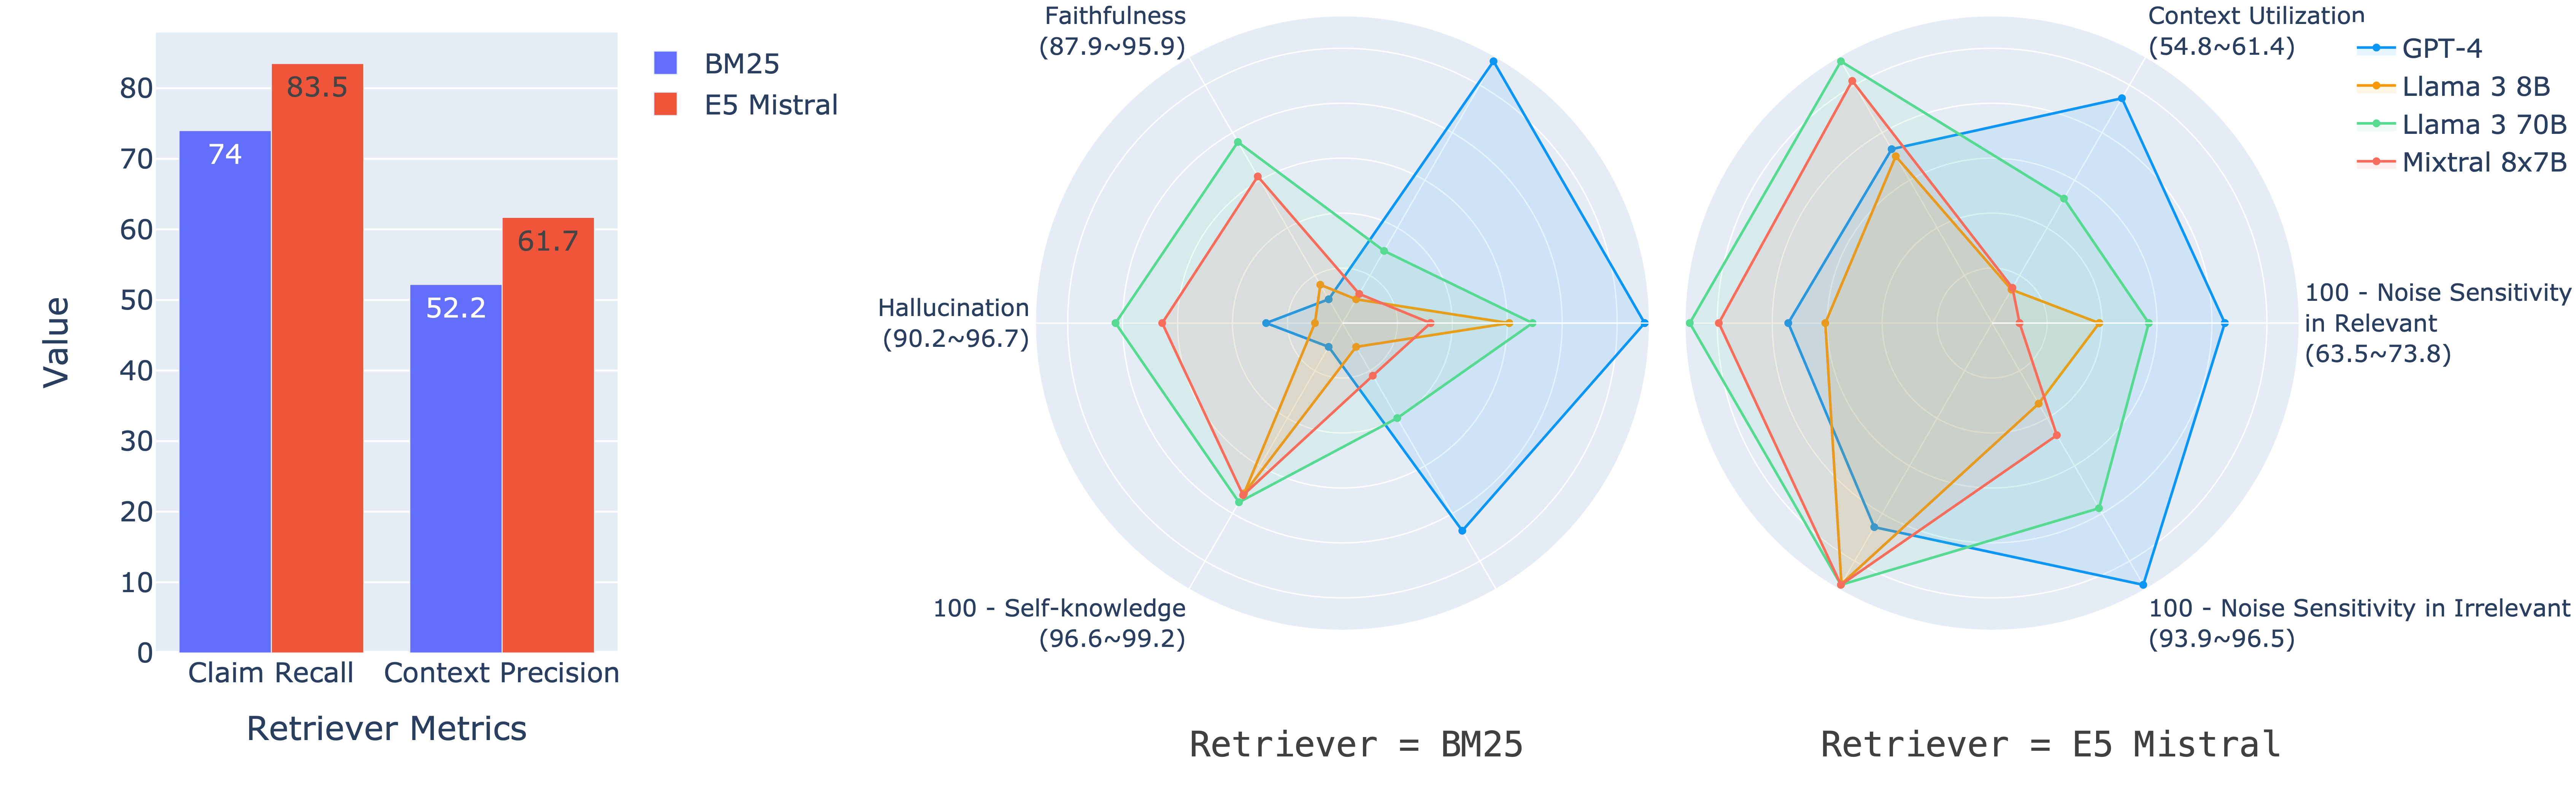
\includegraphics[width=\textwidth]{figures/main_results_avg_radar.png}
%     \caption{Radar charts for BM25 and E5-Mistral retrievers.}
% \end{figure}

\subsection{Diagnosis on RAG Settings for Improvements}
\label{sec:diagnosis_for_imporovements}
Guided by observations in Sec.~\ref{sec:analysis}, we modify settings commonly tuned in RAG systems that may lead to improvements, diagnose their working mechanisms with \benchname\space metrics, and provide suggestions for improvements on certain aspects. We experiment with different numbers of chunks, chunk sizes, chunk overlap ratios, and generation prompts. We highlight our main findings and suggestions as below, please refer to Appendix~\ref{appendix:diagnosis} for detailed analysis and results.

\textbf{More Context Enhances Faithfulness.}
Increasing the number ($k$) and size of chunks improves the recall of more useful information (\emph{claim recall} 61.5$\rightarrow$77.6 with $k$ 5$\rightarrow$20, 70.3$\rightarrow$77.6 with size 150$\rightarrow$300). Consequently, this provides more context for the generators to be more faithful to (\emph{faithfulness} 88.1$\rightarrow$92.2 with $k$ 5$\rightarrow$20, 91.2$\rightarrow$92.2 with size 150$\rightarrow$300), though at the same time they also become more sensitive to additional noise (\emph{noise sensitivity} 34.0$\rightarrow$35.4 with $k$ 5$\rightarrow$20, 34.5$\rightarrow$35.4 with size 150$\rightarrow$300). Improvements in the overall performance (\emph{F1} 51.7$\rightarrow$53.4 with $k$ 5$\rightarrow$20, 52.6$\rightarrow$53.4 with size 150$\rightarrow$300) indicates benefits from more context.

\textbf{Explicit Requirements in Prompts Affect Generation Preferences.}  When prompts introduces explicit requirements for better \emph{faithfulness}, \emph{context utilization}, and lower \emph{noise sensitivity}, generators show improvements in \emph{faithfulness} (92.2$\rightarrow$93.6), but struggle with the subtle tension between \emph{context utilization} (59.2$\rightarrow$63.7) and \emph{noise sensitivity} (35.4$\rightarrow$38.1).

\textbf{Chunk Overlap Does Not Matter a Lot.} The chunk overlap ratio is usually set to be non-zero to help generators better utilize surrounding information and identify chunks with coherent logic. However, it minimally affects generation performance, as retrieving more chunks sharing similar useful information (increased \emph{context precision} 69.3$\rightarrow$71.1) does not necessarily increase the total amount of retrieved useful information (comparable \emph{claim recall} 77.8$\rightarrow$78.1).

\textbf{Suggestions to RAG Builders}

Improving the retriever is an effective way to enhance overall performance. While a better embedding model leads to improvements in both \emph{precision} and \emph{recall}, moderately increasing the number and size of chunks improves \emph{recall} and thus \emph{F1} with minimal efforts in practice. Note that the effect saturates as the total amount of relevant information is fixed, so they need not be too large for a balanced cost-performance. On the other hand, given a limited number of context, larger chunk sizes with fewer chunks are preferred for better \emph{context precision}. However, when targeting better \emph{context utilization} or reduced \emph{noise sensitivity}, opposite adjustments should be made to alleviate the influence of noise.

When tuning the generator, the trilemma of \emph{context utilization}, \emph{noise sensitivity}, and \emph{faithfulness} makes it difficult to improve all aspects simultaneously. RAG builders should prioritize certain aspects in the prompt based on their targets, user preferences and the generator's capability.
